\section{Background}
\subsection{Hopfield Network Elements}
As shown in Figure \ref{fg:HNN1}, Hopfield network consists of a set of interconnected neurons which update their activation values asynchronously. The activation values are binary, usually \{-1,1\}. The update of a unit depends on the other units of the network and on itself. A unit $i$ will be influence by an other unit $j$ with a certain weight $w_{ij}$, and have a threshold value.\\

\begin{figure}[h]
\centering
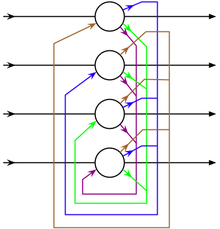
\includegraphics[scale=0.5]{HNN1.png}
\caption{An example of Hopfield Network}
\label{fg:HNN1}
\end{figure}

So there is a constraint due to the other neurons and due the specific threshold of the unit.\\

The new activation value (state) of a neuron is compute, in discrete time, by the function \ref{eq:hop1}:
\begin{equation}
\label{eq:hop1}
x_i(t + 1) = sign(\sum_{j = 1}^{n}x_j(t)w_{ij} - \theta_i)
\end{equation}
or function \ref{eq:hop2}\\
\begin{equation}
\label{eq:hop2}
X = sign(XW - T)
\end{equation}
Where $X$, $W$, $T$ and the $sign$ function are:
\begin{itemize}
  \item $X$ is the activation value of the $n$ units/neurons: $X = \left(\begin{array}{c}
x_1\\ 
x_2\\
\vdots \\
x_n
\end{array}\right)$
  \item $W$ is the weight matrix: $W = \begin{bmatrix}
w_{11} & w_{12} & \dots & w_{1n}  \\
w_{21} & w_{22} & \dots & w_{2n} \\
\vdots  &            & \ddots & \vdots \\
w_{n1} & w_{n2} & \dots & w_{nn} 
\end{bmatrix}$ where $w_{ij}$ can be interpreted as the influence of neuron $i$ over neuron $j$ (and reciprocally).
  \item $T$ is the threshold of each unit: $T = \left(\begin{array}{c}
\theta_{1}\\ 
\theta_2\\
\vdots \\
\theta_{n}
\end{array}\right)$
  \item the $sign$ function is define as function \ref{eq:hop3}:
  \begin{equation}
	\label{eq:hop3}
	sign(x) = \begin{cases}
					+1 & \text{if } x \geq 0\\
					-1 & \text{otherwise}
				\end{cases}
  \end{equation}
\end{itemize}

Usually, an Hopfield Network has a weight matrix symmetric, zero-diagonal(no loop, a unit does not influence on itself). We will only consider that case in our project. 

\subsection{Hebbian Learning}
A simple model due to Donald Hebb captures the idea of associative memory. Imagine that the weights between neurons whose activities are positively correlated are increased:
\begin{equation}
	\label{eq:Heb1}
	\frac{dw_{ij}}{dt} \sim \text{Correlation}(x_i, x_j)
  \end{equation}
  Now imagine that when stimulus $m$ is present (for example, the smell of a banana), the activity of neuron $m$ increases; and that neuron $n$ is associated with another stimulus, $n$ (for example, the sight of a yellow object). If these two stimuli: a yellow sight and a banana smell. co-occur in the environment, then the Hebbian learning rule (\ref{eq:Heb1}) will increase the weights $w_{nm}$ and $w_{mn}$. This means that when, on a later occasion, stimulus $n$ occurs in isolation, making the activity $x_n$ large, the positive weight from $n$ to $m$ will cause neuron $m$ also to be activated. Thus the response to the sight of a yellow object is an automatic association with the smell of a banana. We could call this pattern completion. No teacher is required for this associative memory to work. No signal is needed to indicate that a correlation has been detected or that an association should be made. The unsupervised, local learning algorithm and the unsupervised, local activity rule spontaneously produce associative memory.\\

  Similar with the example above, we could imagine each standard character image as a complete graph which is shown in Figure \ref{fg:HNN2}. Each pixel in the image will be the neuron in Hopfield Network. We will use the idea of Hebbian learning to train the network which will change weights between each pair of neuron in the network.\\
  \begin{figure}[h]
  \centering
  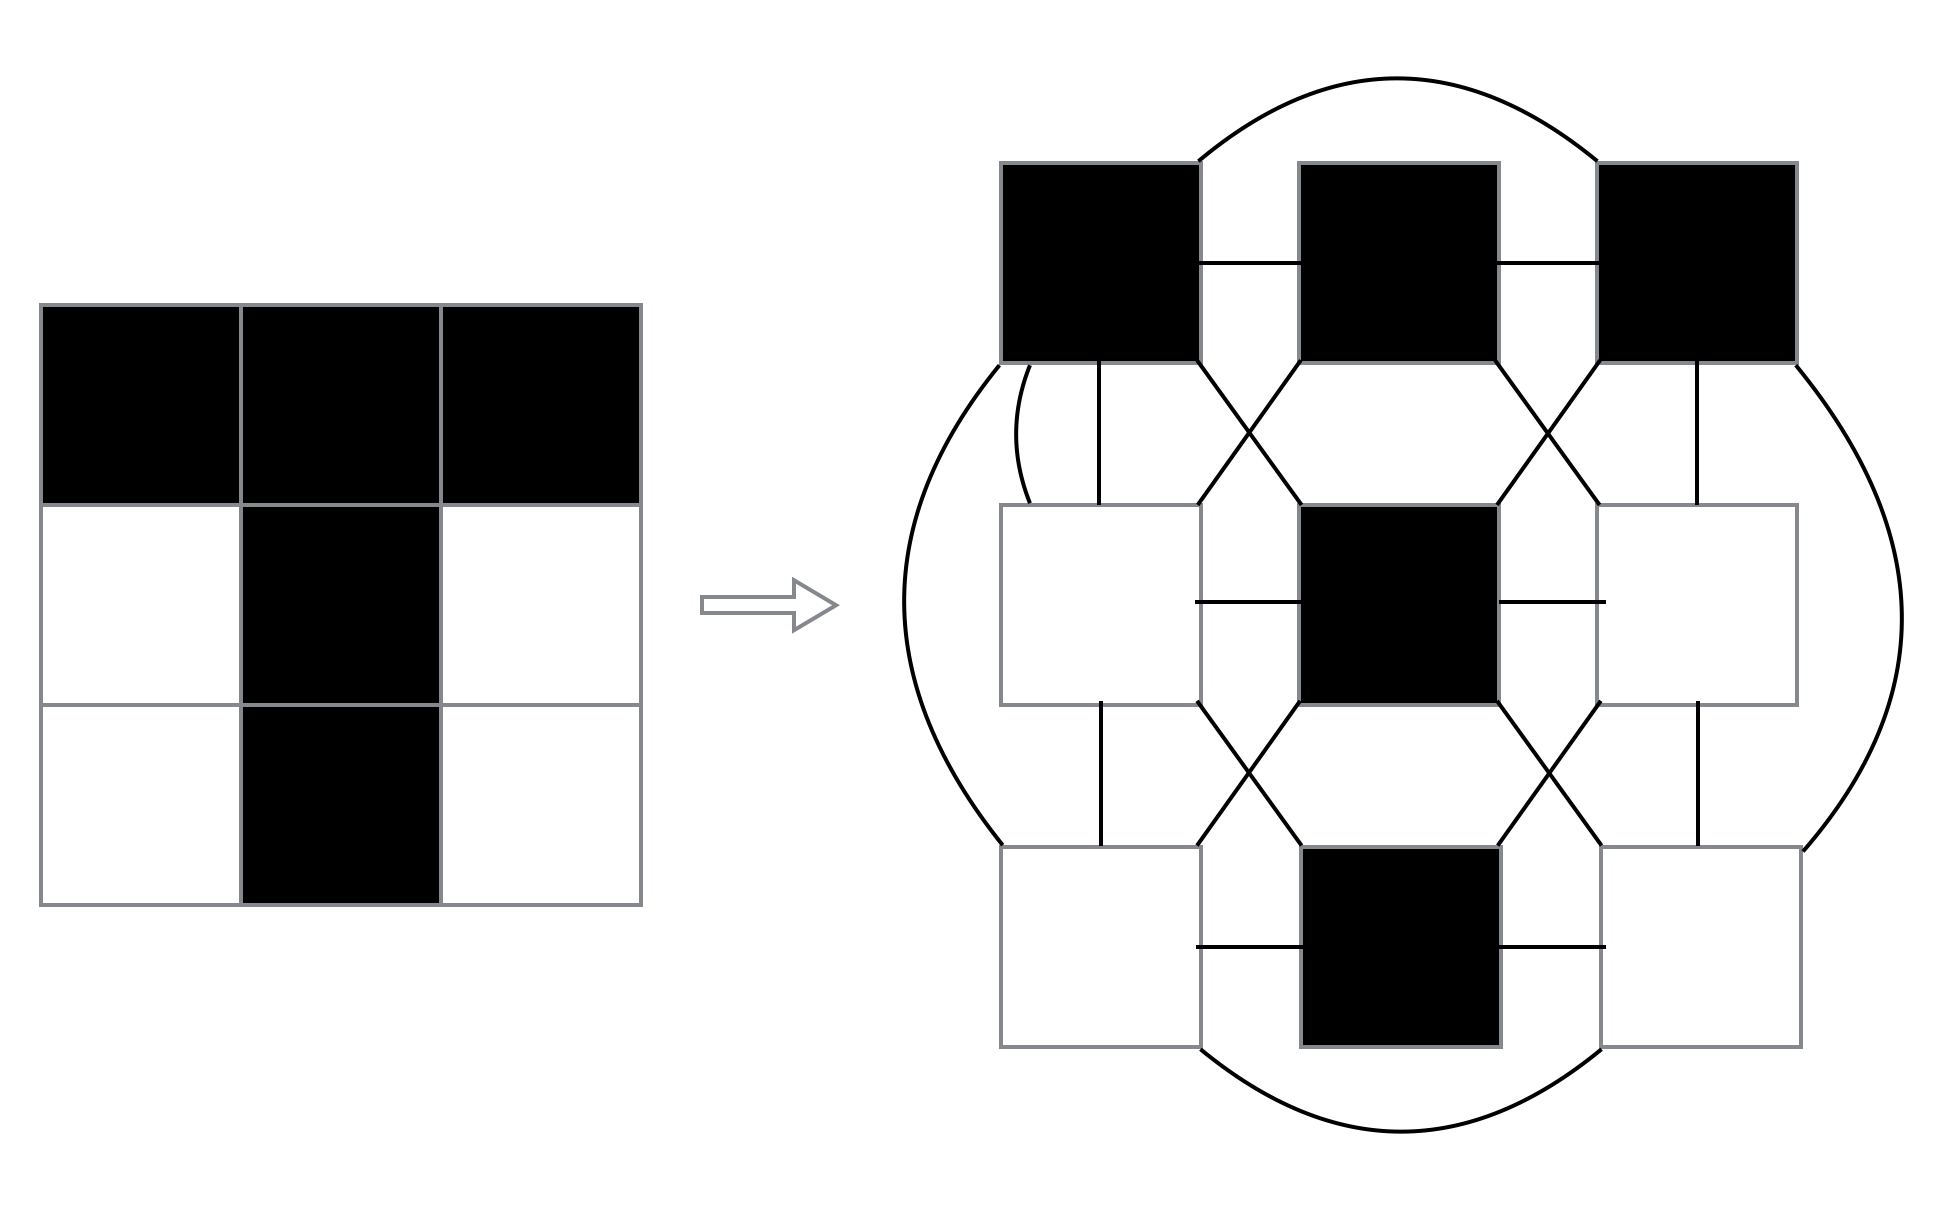
\includegraphics[scale=0.3]{HNN2.png}
  \caption{Character $T$ being denoted as Hopfield Network}
  \label{fg:HNN2}
  \end{figure}

  In the Hebbian learning, the weight of the matrix results from a unsupervised learning, this learning type is a reinforcement learning. We consider that we can ”impress” patterns to the network in order to recognize one of them even if they are given in input with a lot of noise. The learning phase consists in learning different pattern in order to set the weight of the edges. For each pattern, we can resume the learning phase as:
  \begin{itemize}
    \item If two unit has the same activation state (\{1, 1\} or \{-1, -1\}), the strength of the connection is reinforce($w_{ij}$ increase).
    \item If two unit has opposite activation state (\{-1, 1\}), the strength of the connection decline.
  \end{itemize}
  With those kind of rule, $W$ will store patterns and then allow the network to converge to them. Unfortunately, in that case we can not predict the convergence to the right pattern (the network will still converge but we cannot predict to which stable state). \\

  The weight matrix is modified according to the $m$ pattern we want to store. Those pattern represent the stable state we hope to reach. The weights are modified, for example:
  \begin{equation}
  \label{eq:Heb2}
  w_{ij}' = w_{ij} + \epsilon x_i x_j
  \end{equation}
  Equation \ref{eq:Heb2} is iterated various time for each pattern. $x_i$ and $x_j$ represent the state of the units $i$ and $j$ of the pattern being learned. $\epsilon$ is a constant to prevent the connection to became to big or to small(For example: $\epsilon = \frac{1}{m}$)\\

  When $m = 1$, we always converge to the impress pattern. When $m > 1$, we can only hope to converge to a known pattern if the different patterns are as orthogonal as possible (the different patterns have to be really different). If they are quite related it is possible to have a mix of different pattern.

  We can increase the capacity of our network by modifying our objective function to measure how well it stores memories and minimizing that function. Consider the error between a single neuron of the network, with inputs $\textbf{x}^{(n)}$ and binary labels $t^{(n)}$. We can define this error function $G(W)$ as follows:
\begin{equation}
\label{eq:opt1}
G(W) = -\sum_{i} \sum_{n} t_{i}^{(n)}\text{ln}y_{i}^{(n)} + (1 - t_{i}^{n})\text{ln}(1 - y_{i}^{(n)})
\end{equation}

where

\begin{equation}
\label{eq:opt2}
t_{i}^{(n)} = \begin{cases}
          1 & x_{i}^{(n)} = 1\\
          0 & x_{i}^{(n)} = -1
        \end{cases}
\end{equation}

and

\begin{equation}
\label{eq:opt3}
y_{i}^{(n)} = \frac{1}{1 + e^{-a_{i}^{(n)}}}
% y_{i}^{(n)} = \frac{1}{1 + e^{-a_{i}^{(n)}}} & \text{where a_{i}^{n} = \sum w_{ij}x_{j}^{(n)}}
\end{equation}

Now we can minimize $G(W)$ to determine our weights. However, we run the risk of over fitting our network. We will reduce this risk by making use of regularization. In this case we will minimize 
\begin{equation}
\label{eq:opt4}
M(W) = G(W) + \alpha E_w(W)
\end{equation}
where $\alpha$ is a regularization parameter and $E_w(W)$ is a penalty function. it will act as a bias against $W$ which will keep the values from becoming too large and over-fitting the data.\\

We will be minimizing the function by utilizing gradient descent, a first order optimization algorithm. Gradient descent works via a back-propagation algorithm whereby we modify $w$ to move opposite the gradient of $G$. In this way we find the $w$ which minimizes the error function.


\subsection{Convergence of Hopfield Network}
Hopfield networks converges to a local state. The energy function of a Hopfield network in a certain state is:
\begin{equation}
\label{eq:energy1}
E_1 = \frac{1}{2}X^tWX + TX^t = - \frac{1}{2}\sum_{i = 1}^{n}\sum_{j = 1}^{n}w_{ij} x_i x_j + \sum_{i = 1}^n \theta_i x_i
\end{equation}

\begin{equation}
\label{eq:energy2}
E_2 = \frac{1}{2}X^tWX = - \frac{1}{2}\sum_{i = 1}^{n}\sum_{j = 1}^{n}w_{ij} x_i x_j
\end{equation}
Equation \ref{eq:energy1} can be useful as a general energy function. More often, we use equation \ref{eq:energy2}. Equation \ref{eq:energy2} is equivalent to equation \ref{eq:energy1}.\\

In order to take into account the threshold of the units, we add a artificial unit which is in the activation state 1. This unit is linked to the other with the value of their negative threshold. In that case, the new weight matrix will be
\begin{equation}
\label{eq:energy3}
W_G = \begin{bmatrix}W & T \\T^t & 0 \end{bmatrix}
\end{equation}
Those energy functions are helpful to determinate the actual state of the network.\\

As the dynamic is asynchronous, only one unit is evaluated at each time. If the $k^{th}$ unit is selected, there is two options:

\begin{enumerate}
  \item $k$ does not change state
  \item $k$ changes 
\end{enumerate}
In the first case, the energy function remains the same, $E(t + 1) = E(t)$. Otherwise, the energy function changes, according to the new excitation value $(x'_k)$ of the $k^{th}$ unit. The difference of energy of the system is given by:
\begin{equation}
\label{eq:energy4}
E_1(x) - E_1(x') = (-\sum_{j = 1}^{n}w_{kj} x_j x_k + \theta_k x_k) - (-\sum_{j = 1}^{n} w_{kj} x_j x'_k + \theta_k x'_{k})
\end{equation}
Then we have:
\begin{equation}
\label{eq:energy5}
E_1(x) - E_1(x') = -(x_k - x'_k) \cdot (\sum_{j = 1}^{n} w_{kj}x_j - \theta_k)
\end{equation}
The second term of equation \ref{eq:energy5}: ($\sum_{j = 1}^{n} w_{kj}x_j - \theta_k$) is the excitation $e_k$ of the $k^{th}$ unit. The unit changed its state, so the excitation has a different sign than $x_k$ and $-x'_k$ (according to equation \ref{eq:hop1}). Therefore, $E_1(x) - E_1(x')$ is positive, which implies that $E(x) > E(x')$.  So the energy will decrease for every change, and since there is only a finite number of possible states, the network should reach a state where the energy cannot decrease more, it will be a stable state.\\

Of course the stable state is not unique but it is certain that the system will converge. The final state will depend on the input, the initial state of the system. This conclusion is very useful since we could first train the Hopfield network to get multiple stable state that stand for specific character or digits. Then the input image will be handwritten character or digits with noise and they will be expected to converge to a stable state that we trained previously. \\

